\chapter{EXPERIMENTAL RESULTS}
\label{ch:Experimental Results}
In this chapter we show the experiments we have made and their results.

The four experiments we talk about here are the following:
\begin{itemize}
 \item Experiment 1: Why use torque values instead of force.
 \item Experiment 2: Minimum radius of the pivot.
 \item Experiment 3: Minimum distance between pivots.
 \item Experiment 4: Comparison of robot fail ratio with human fail ratio.
\end{itemize}

The first experiment explains why we used torque values in this work instead of force values to determine the direction of string tension. We also explain how the threshold value for torque has been established.

The second experiment shows which is the minimum radius for the pivot to distinguish between CW and CCW case. We establish the minimum radius from which the pivot is considered negligible.

The third experiment consists on establishing the minimum distance between pivots to distinguish them through torque values.

Finally, the fourth experiment consists on comparing robot fail ratio with human fail ratio. There we do several experiments with the robot, and then we repeat the same experiments with different people in the same conditions than the robot (with no vision).

Let's start explaining the first experiment.

\section{Experiment 1: Why use torque values instead of force}
As told before, here we explain why we use torques instead of forces and then we establish the threshold from which torque values are considered relevant.

\subsection{Comparison between force values and torque values}
It is true that the most intuitive way to solve the problem of untying the string from the pivot would be to look at forces because these would directly tell the direction of string tension. But, let's see what happens if we look to force and torque readings of the Robotiq FT300 sensor in the case where there is no tension of the string and in the case where there is.

For this experiment, the case of no string tension is the initial pose, when the gripper is just grasping the end of the string between the two pivots, before starting the movement. The case of string tension is the case when the gripper moves $2 \cdot r_{p}$ in perpendicular to pivots joining axis. Figure~\ref{fig:exp1} below shows both cases.
\begin{figure}[h!]
	\centering
	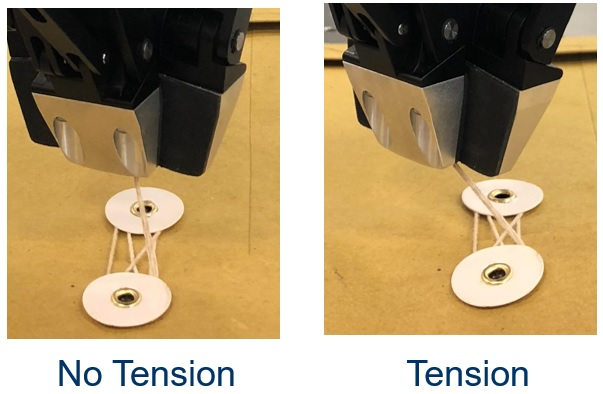
\includegraphics[height=60mm]{chapters/figures/experiments/exp1.jpg}
	\caption{Tension and No Tension cases.}
	\label{fig:exp1}
\end{figure}

Let's take 30 values of force and torque from the force/torque sensor in both cases. Results are presented in Table~\ref{tab:readings}.%\clearpage
% Table generated by Excel2LaTeX from sheet 'CW P1'
%\begin{longtable}[htbp]
%\begin{center}
\setlength\LTpost{0pt}
\begin{longtable}{|c|c|c|c|rr|c|c|c|c|}
		\cmidrule{1-4}\cmidrule{7-10}    \multicolumn{4}{|c|}{\textbf{NO TENSION (INITIAL POSE)}} &       &       & \multicolumn{4}{c|}{\textbf{TENSION (CW P1)}} \\
		\cmidrule{1-4}\cmidrule{7-10}    \textbf{$F_{x} (N)$} & \textbf{$F_{y} (N)$} & \textbf{$M_{x} (N \cdot m)$} & \textbf{$M_{y} (N \cdot m)$} &       &       & \textbf{$F_{x} (N)$} & \textbf{$F_{y} (N)$} & \textbf{$M_{x} (N \cdot m)$} & \textbf{$M_{y} (N \cdot m)$} \\
		\cmidrule{1-4}\cmidrule{7-10}    1.19  & 1.41  & 0.072 & 0.032 &       &       & 2.55  & -0.04 & -0.177 & 0.422 \\
		0.76  & 0.27  & 0.023 & 0.035 &       &       & 2.81  & 1.56  & -0.199 & 0.431 \\
		-0.04 & -0.19 & 0.060 & 0.007 &       &       & 2.25  & -0.40 & -0.194 & 0.432 \\
		0.13  & -1.28 & 0.057 & 0.006 &       &       & 2.34  & 0.06  & -0.170 & 0.412 \\
		1.96  & 0.13  & 0.056 & 0.030 &       &       & 3.31  & -1.18 & -0.184 & 0.422 \\
		0.71  & -0.63 & 0.033 & 0.037 &       &       & 3.75  & 1.00  & -0.215 & 0.440 \\
		1.61  & -0.26 & 0.043 & 0.045 &       &       & 2.71  & 1.00  & -0.214 & 0.446 \\
		1.79  & -0.90 & 0.056 & 0.010 &       &       & 3.96  & 1.24  & -0.214 & 0.434 \\
		0.13  & 0.28  & 0.049 & 0.039 &       &       & 3.28  & 2.52  & -0.190 & 0.411 \\
		-0.65 & 0.31  & 0.009 & 0.044 &       &       & 5.23  & -0.31 & -0.196 & 0.448 \\
		-0.88 & -0.81 & 0.063 & 0.045 &       &       & 2.18  & -0.44 & -0.212 & 0.425 \\
		-0.36 & 1.10  & 0.069 & 0.014 &       &       & 3.60  & 1.04  & -0.198 & 0.411 \\
		0.43  & -0.49 & 0.056 & 0.049 &       &       & 3.47  & 2.06  & -0.191 & 0.406 \\
		-0.64 & -0.10 & 0.065 & 0.029 &       &       & 2.41  & 0.46  & -0.157 & 0.430 \\
		0.50  & -0.22 & 0.058 & 0.032 &       &       & 3.65  & 1.72  & -0.169 & 0.416 \\
		-0.42 & -0.89 & 0.067 & 0.031 &       &       & 3.04  & -0.91 & -0.191 & 0.409 \\
		0.15  & -1.66 & 0.074 & 0.020 &       &       & 3.23  & 0.08  & -0.177 & 0.403 \\
		-0.74 & 0.89  & 0.074 & 0.028 &       &       & 3.18  & 1.10  & -0.190 & 0.415 \\
		1.38  & -1.86 & 0.071 & 0.037 &       &       & 4.07  & 0.63  & -0.192 & 0.407 \\
		0.21  & -1.05 & 0.073 & 0.048 &       &       & 4.28  & -0.57 & -0.197 & 0.428 \\
		0.26  & -0.95 & 0.072 & 0.022 &       &       & 3.86  & 0.14  & -0.207 & 0.390 \\
		0.38  & -1.54 & 0.061 & 0.035 &       &       & 3.26  & -1.17 & -0.188 & 0.442 \\
		1.43  & -2.17 & 0.058 & 0.057 &       &       & 3.17  & 0.10  & -0.199 & 0.368 \\
		0.16  & -0.71 & 0.013 & 0.058 &       &       & 3.05  & 0.06  & -0.173 & 0.438 \\
		-0.67 & -0.21 & 0.078 & 0.045 &       &       & 4.87  & 1.35  & -0.182 & 0.444 \\
		0.21  & -1.97 & 0.065 & 0.021 &       &       & 2.30  & 0.67  & -0.155 & 0.403 \\
		0.06  & -0.46 & 0.063 & 0.001 &       &       & 3.23  & 3.23  & -0.200 & 0.409 \\
		1.43  & -1.37 & 0.044 & 0.026 &       &       & 4.64  & -0.95 & -0.180 & 0.417 \\
		-1.43 & -0.77 & 0.042 & 0.049 &       &       & 3.67  & 2.00  & -0.171 & 0.407 \\
		1.08  & -0.83 & 0.073 & 0.015 &       &       & 1.12  & -0.19 & -0.199 & 0.430 \\
		\cmidrule{1-4}\cmidrule{7-10}    %\end{longtable}%
	\caption{Results of force and torque readings for the case of no tension and the case of tension of the string.}
	\label{tab:readings}%
\end{longtable}% 
%\end{center}% 

Now let's look to the maximum and minimum values in each case (Table~\ref{tab:maxmin}).
% Table generated by Excel2LaTeX from sheet 'CW P1'
% Table generated by Excel2LaTeX from sheet 'CW P1'
\begin{table}[htbp]
	\centering
	\begin{tabular}{l|c|c|c|c|c|c|c|c|}
		\cmidrule{2-9}
		& \multicolumn{4}{c|}{\textbf{NO TENSION (INITIAL POSE)}} & \multicolumn{4}{c|}{\textbf{TENSION (CW P1)}} \\
		\cmidrule{2-9}
		\multicolumn{1}{r|}{} & \textbf{$F_{x} (N)$} & \textbf{$F_{y} (N)$} & \textbf{$M_{x} (N \cdot m)$} & \textbf{$M_{y} (N \cdot m)$} & \textbf{$F_{x} (N)$} & \textbf{$F_{y} (N)$} & \textbf{$M_{x} (N \cdot m)$} & \textbf{$M_{y} (N \cdot m)$} \\
		\midrule
		\multicolumn{1}{|l|}{\textbf{Min}} & -1.43 & -2.17 & 0.009 & 0.001 & 1.12  & -1.18 & -0.215 & 0.368 \\
		\midrule
		\multicolumn{1}{|l|}{\textbf{Max}} & 1.96  & 1.41  & 0.078 & 0.058 & 5.23  & 3.23  & -0.155 & 0.448 \\
		\midrule
		\multicolumn{1}{|l|}{\textbf{Max - Min}} & 3.39  & 3.58  & 0.069 & 0.057 & 4.11  & 4.41  & 0.060 & 0.080 \\
		\bottomrule
	\end{tabular}%
	\caption{Maximum and minimum values of force and torque.}
	\label{tab:maxmin}%
\end{table}%

We appreciate that the difference between the maximum and the minimum value for force readings is around $4 N$, while for torques it is around $0.070 N \cdot m$. The sensor is much noisier for force readings than for torques. Furthermore, if we compare maximum and minimum values in \textit{tension} and \textit{no tension} case, we see that force values are overlapped in both cases:
\[ F_{x, max, no tension} = 1.96 N > 1.12 N = F_{x, min, tension} \]
\[ F_{y, max, no tension} = 1.41 N > -1.18 N = F_{y, min, tension} \]

While torques are clearly distinguishable:
\[ M_{x, min, no tension} = 0.009 N\cdot m > -0.155 N\cdot m = M_{x, max, tension} \]
\[ M_{y, max, no tension} = 0.058 N\cdot m < 0.368 N\cdot m = M_{y, min, tension} \]

As there is an error in sensor readings, we decided to take the mean values as the most accurates values to compare both cases. Let's look now to mean values and standard deviation in Table~\ref{tab:mean}.
% Table generated by Excel2LaTeX from sheet 'CW P1'
%\begin{table}[htbp]
%	\centering
%	\begin{tabular}{|l|c|c|c|c|c|}
\setlength\LTpost{0pt}
\begin{longtable}{|l|c|c|c|c|c|}
		\multicolumn{1}{|r}{} &       & \textbf{$F_{x} (N)$} & \textbf{$F_{y} (N)$} & \textbf{$M_{x} (N \cdot m)$} & \textbf{$M_{y} (N \cdot m)$} \\
		\midrule
		\multicolumn{1}{|p{9.125em}|}{\textbf{NO TENSION}} & St. dev. & 0.86  & 0.89  & 0.018  & 0.015 \\
		\cmidrule{2-6}    \textbf{(INITIAL POSE)} & Mean  & 0.34  & -0.56 & 0.057  & 0.032 \\
		\midrule
		\multicolumn{1}{|p{9.125em}|}{\textbf{TENSION}} & St. dev. & 0.87  & 1.12  & 0.016  & 0.018 \\
		\cmidrule{2-6}    \textbf{(CW P1)} & Mean  & 0.49  & 0.53  & -0.189 & 0.42 \\
		\bottomrule
%	\end{tabular}%
	\caption{Standard deviation and mean values for force and torque readings in tension and no tension case.}
	\label{tab:mean}%
\end{longtable}%

With this values of standard deviation and mean, we establish the ranges of force and torque variations for tension and no tension case. The results are shown in Table~\ref{tab:ranges}.
% Table generated by Excel2LaTeX from sheet 'CW P1'
%\begin{table}[htbp]
%	\centering
%	\setlength\LTpre{0pt}
\setlength\LTpost{0pt}
\begin{longtable}{|c|c|c|}
		\cmidrule{2-3}    \multicolumn{1}{c|}{} & \multicolumn{1}{p{12.915em}|}{\textbf{No Tension (Initial pose)}} & \multicolumn{1}{p{12.915em}|}{\textbf{Tension case (CW P1)}} \\
		\midrule
		\textbf{$F_{x} \pm st. dev. (N)$} & $-0.52 N < F_{x} < 1.2 N$ & $-0.38 N < F_{x} < 1.36 N$ \\
		\midrule
		\textbf{$F_{y} \pm st. dev. (N)$} & $-1.45 N < F_{y} < 0.33 N$ & $-0.59 N < F_{y} < 1.65 N$ \\
		\midrule
		\textbf{$M_{x} \pm st. dev. (N \cdot m)$} & $0.039 N \cdot m < M_{x} < 0.075 N \cdot m$ & $-0.205 N \dot m < M_{x} < -0.173 N \cdot m$ \\
		\midrule
		\textbf{$M_{y} \pm st. dev. (N \cdot m)$} & $0.017 N \cdot m < M_{y} < 0.047 N \cdot m$ & $0.402 N \cdot m < M_{y} < 0.438 N \cdot m$ \\
		\bottomrule
%	\end{longtable}%
	\caption{Ranges of force and torque variations in tension and no tension cases.}
	\label{tab:ranges}%
\end{longtable}%

Looking to forces values, we see that both ranges for $F_{x}$ and $F_{y}$ are overlapped in case of tension and no tension. Variation in force readings is too big compared to the little forces (tension of the string) we are working with. We can thus not distinguish between the tension case and no tension case with force values. Force cannot be used to determine the direction of string tension in this case.

Otherwise, if we look to torque values, we see that ranges for tension case and no tension case are clearly distinguishable. Torque readings are much more precise than force readings and that is why we use torque values in this work.

\subsection{Threshold value for torque}
After explaining why torque values are more accurate for this project, let's establish now the threshold value for torque readings to be considered relevant. 

To  do that, we made 10 experiments where we took 30 values of torque in tension and in no tension case. Then, with the mean and the standard deviation we compare both cases of each experiment. We show directly the results for the mean and standard deviation in each experiment. These are shown in Table~\ref{tab:experimenttorques} below:
% Table generated by Excel2LaTeX from sheet 'CW P1'
\setlength\LTpost{0pt}
\begin{longtable}{|r|c|c|c|c|c|}
		\cmidrule{3-6}    \multicolumn{1}{r}{} &       & \multicolumn{2}{c|}{\textbf{NO TENSION (INITIAL POSE)}} & \multicolumn{2}{c|}{\textbf{TENSION (CW P1)}} \\
		\cmidrule{3-6}    \multicolumn{1}{r}{} &       & \textbf{St. dev.} & \textbf{Mean} & \textbf{St. dev.} & \textbf{Mean} \\
		\midrule
		\multicolumn{1}{|l|}{\textbf{Experiment 1}} & \textbf{$M_{x} (N \cdot m)$} & 0.018 & 0.057 & 0.016 & -0.189 \\
		\cmidrule{2-6}          & \textbf{$M_{y} (N \cdot m)$} & 0.015 & 0.032 & 0.018 & 0.42 \\
		\midrule
		\multicolumn{1}{|l|}{\textbf{Experiment 2}} & \textbf{$M_{x} (N \cdot m)$} & 0.022 & 0.042 & 0.021 & -0.168 \\
		\cmidrule{2-6}          & \textbf{$M_{y} (N \cdot m)$} & 0.016 & 0.033 & 0.026 & 0.140 \\
		\midrule
		\multicolumn{1}{|l|}{\textbf{Experiment 3}} & \textbf{$M_{x} (N \cdot m)$} & 0.017 & 0.028 & 0.024 & -0.072 \\
		\cmidrule{2-6}          & \textbf{$M_{y} (N \cdot m)$} & 0.024 & 0.042 & 0.022 & 0.184 \\
		\midrule
		\multicolumn{1}{|l|}{\textbf{Experiment 4}} & \textbf{$M_{x} (N \cdot m)$} & 0.019 & 0.052 & 0.024 & -0.056 \\
		\cmidrule{2-6}          & \textbf{$M_{y} (N \cdot m)$} & 0.014 & 0.047 & 0.015 & 0.143 \\
		\midrule
		\multicolumn{1}{|l|}{\textbf{Experiment 5}} & \textbf{$M_{x} (N \cdot m)$} & 0.015 & 0.031 & 0.018 & -0.173 \\
		\cmidrule{2-6}          & \textbf{$M_{y} (N \cdot m)$} & 0.022 & 0.022 & 0.019 & 0.215 \\
		\midrule
		\multicolumn{1}{|l|}{\textbf{Experiment 6}} & \textbf{$M_{x} (N \cdot m)$} & 0.016 & 0.009 & 0.024 & -0.240 \\
		\cmidrule{2-6}          & \textbf{$M_{y} (N \cdot m)$} & 0.015 & 0.020 & 0.016 & 0.199 \\
		\cmidrule{1-1}\cmidrule{3-6}    \multicolumn{1}{|l|}{\textbf{Experiment 7}} & \textbf{$M_{x} (N \cdot m)$} & 0.021 & 0.053 & 0.020 & -0.291 \\
		\cmidrule{2-6}          & \textbf{$M_{y} (N \cdot m)$} & 0.028 & 0.045 & 0.023 & 0.284 \\
		\midrule
		\multicolumn{1}{|l|}{\textbf{Experiment 8}} & \textbf{$M_{x} (N \cdot m)$} & 0.028 & 0.055 & 0.016 & -0.078 \\
		\cmidrule{2-6}          & \textbf{$M_{y} (N \cdot m)$} & 0.021 & 0.031 & 0.011 & 0.152 \\
		\midrule
		\multicolumn{1}{|l|}{\textbf{Experiment 9}} & \textbf{$M_{x} (N \cdot m)$} & 0.026 & 0.038 & 0.018 & -0.085 \\
		\cmidrule{2-6}          & \textbf{$M_{y} (N \cdot m)$} & 0.015 & 0.017 & 0.021 & 0.141 \\
		\midrule
		\multicolumn{1}{|l|}{\textbf{Experiment 10}} & \textbf{$M_{x} (N \cdot m)$} & 0.023 & 0.053 & 0.021 & -0.115 \\
		\cmidrule{2-6}          & \textbf{$M_{y} (N \cdot m)$} & 0.027 & 0.056 & 0.018 & 0.202 \\
		\bottomrule
		\caption{Results for 10 experiments of standard deviation and mean values for torque in tension and no tension case.}
		\label{tab:experimenttorques}%
\end{longtable}%

The maximum value of standard deviation is $0.028 N\cdot m$ in experiments 7 and 8, so the threshold value must be greater than $0.028 N\cdot m$. 

To see if any torque value is overlapped in tension and no tension case, let's establish the ranges of variation of torque in each experiment. These ranges are shown in  Table~\ref{tab:rangetorques}:
% Table generated by Excel2LaTeX from sheet 'CW P1'
\setlength\LTpost{0pt}
\begin{longtable} {|r|c|c|c|c|c|}
		\cmidrule{3-4}    \multicolumn{1}{r}{} &       & \textbf{NO TENSION (INITIAL POSE)} & \textbf{TENSION (CW P1)} \\
		\midrule
		\multicolumn{1}{|l|}{\textbf{Exp. 1}} & \textbf{$M_{x} \pm st. dev. (N \cdot m)$} & $0.039 < M_{x} < 0.075$ & $-0.205 < M_{x} < -0.173 $ \\
		& \textbf{$M_{y} \pm st. dev. (N \cdot m)$} & $0.017 < M_{y} < 0.047$ & $0.402 < M_{y} < 0.438$ \\
		\cmidrule{1-4}
		\multicolumn{1}{|l|}{\textbf{Exp. 2}} & \textbf{$M_{x} \pm st. dev. (N \cdot m)$} & $0.02 < M_{x} < 0.064$ & $-0.189 < M_{x} < -0.147$ \\
		& \textbf{$M_{y} \pm st. dev. (N \cdot m)$} & $0.017 < M_{y} < 0.049$ & $0.114 < M_{y} < 0.166$ \\
		\cmidrule{1-4}
		\multicolumn{1}{|l|}{\textbf{Exp. 3}} & \textbf{$M_{x} \pm st. dev. (N \cdot m)$} & $0.011 < M_{x} < 0.045$ & $-0.096 < M_{x} < -0.048$ \\
		& \textbf{$M_{y} \pm st. dev. (N \cdot m)$} & $0.018 < M_{y} < 0.066$ & $0.162 < M_{y} < 0.206$ \\
		\cmidrule{1-4}
		\multicolumn{1}{|l|}{\textbf{Exp. 4}} & \textbf{$M_{x} \pm st. dev. (N \cdot m)$} & $0.033 < M_{x} < 0.071$ & $-0.08 < M_{x} < -0.032$ \\
		& \textbf{$M_{y} \pm st. dev. (N \cdot m)$} & $0.033 < M_{y} < 0.061$ & $0.128 < M_{y} < 0.158$ \\
		\cmidrule{1-4}
		\multicolumn{1}{|l|}{\textbf{Exp. 5}} & \textbf{$M_{x} \pm st. dev. (N \cdot m)$} & $0.016 < M_{x} < 0.046$ & $-0.191 < M_{x} < -0.155$ \\
		& \textbf{$M_{y} \pm st. dev. (N \cdot m)$} & $0.000 < M_{y} < 0.044$ & $0.196 < M_{y} < 0.234$ \\
		\cmidrule{1-4}
		\multicolumn{1}{|l|}{\textbf{Exp. 6}} & \textbf{$M_{x} \pm st. dev. (N \cdot m)$} & $-0.007 < M_{x} < 0.025$ & $-0.264 < M_{x} < -0.216$ \\
		& \textbf{$M_{y} \pm st. dev. (N \cdot m)$} & $0.005 < M_{y} < 0.035$ & $0.183 < M_{y} < 0.215$ \\
		\cmidrule{1-4}
		\multicolumn{1}{|l|}{\textbf{Exp. 7}} & \textbf{$M_{x} \pm st. dev. (N \cdot m)$} & $0.032 < M_{x} < 0.074$ & $-0.311 < M_{x} < -0.271$ \\
		& \textbf{$M_{y} \pm st. dev. (N \cdot m)$} & $0.017 < M_{y} < 0.073$ & $0.261 < M_{y} < 0.307$ \\
		\cmidrule{1-4}
		\multicolumn{1}{|l|}{\textbf{Exp. 8}} & \textbf{$M_{x} \pm st. dev. (N \cdot m)$} & $0.027 < M_{x} < 0.083$ & $-0.094 < M_{x} < -0.062$ \\
		& \textbf{$M_{y} \pm st. dev. (N \cdot m)$} & $0.010 < M_{y} < 0.052$ & $0.141 < M_{y} < 0.163$ \\
		\cmidrule{1-4}
		\multicolumn{1}{|l|}{\textbf{Exp. 9}} & \textbf{$M_{x} \pm st. dev. (N \cdot m)$} & $0.012 < M_{x} < 0.064$ & $-0.103 < M_{x} < -0.067$ \\
		& \textbf{$M_{y} \pm st. dev. (N \cdot m)$} & $0.002 < M_{y} < 0.032$ & $0.120 < M_{y} < 0.162$ \\
		\cmidrule{1-4}
		\multicolumn{1}{|l|}{\textbf{Exp. 10}} & \textbf{$M_{x} \pm st. dev. (N \cdot m)$} & $0.030 < M_{x} < 0.076$ & $-0.136 < M_{x} < -0.094$ \\
		& \textbf{$M_{y} \pm st. dev. (N \cdot m)$} & $0.029 < M_{y} < 0.083$ & $0.184 < M_{y} < 0.220$ \\
		\bottomrule
	\caption{Range of variation of torques in 10 experiments.}
	\label{tab:rangetorques}%
\end{longtable}%

We appreciate that in the 10 experiments, ranges in tension case and in no tension case are never overlapped. 

Finally, we look to the difference between the means of both cases in each experiment (Table~\ref{tab:meandifference}).
% Table generated by Excel2LaTeX from sheet 'CW P1'
\begin{table}[htbp]
	\centering
	\begin{tabular}{|l|c|c|}
		\cmidrule{2-3}    \multicolumn{1}{r|}{} & \textbf{$M_{x, tension} - M_{x, no tension} (N \cdot m)$} & \textbf{$M_{y, tension} - M_{y, no tension} (N \cdot m)$} \\
		\midrule 
		\textbf{Experiment 1} & -0.246 & 0.388 \\
		\midrule
		\textbf{Experiment 2} & -0.21 & 0.107 \\
		\midrule
		\textbf{Experiment 3} & -0.100 & 0.142 \\
		\midrule
		\textbf{Experiment 4} & -0.108 & 0.096 \\
		\midrule
		\textbf{Experiment 5} & -0.204 & 0.193 \\
		\midrule
		\textbf{Experiment 6} & -0.249 & 0.179 \\
		\midrule
		\textbf{Experiment 7} & -0.344 & 0.239 \\
		\midrule
		\textbf{Experiment 8} & -0.133 & 0.121 \\
		\midrule
		\textbf{Experiment 9} & -0.123 & 0.124 \\
		\midrule
		\textbf{Experiment 10} & -0.168 & 0.146 \\
		\bottomrule
	\end{tabular}%
	\caption{Difference between means in tension and no tension case for 10 experiments.}
	\label{tab:meandifference}%
\end{table}%

We appreciate that the minimum difference between the 2 cases is for $M_{y}$ in experiment 4, and the value is $0.096 N \cdot m$. We decided thus, to establish a threshold value of \textbf{$0.095 N \cdot m$} from which we consider that the string is taut. Furthermore, this value is greater than $0.028 N\cdot m$, which is the maximum standard deviation. 

\section{Experiment 2: Minimum radius of the pivots}
In this section we show the experiment made to figure out which is the minimum radius of the pivots for the sensor to distinguish between CW and CCW case.

For this, we took different objects with different radius and we wound the thread around them. By moving $2 \cdot r_{p}$, we see when torque values do not allow to distinguish anymore between CW and CCW case.

\subsection{Radius = 4 mm}
We start with the real radius of our pivots. This is 4 mm. In Figure~\ref{fig:CWCCW1} below, we can see the difference between CW and CCW case:
\begin{figure}[h!]
	\centering
	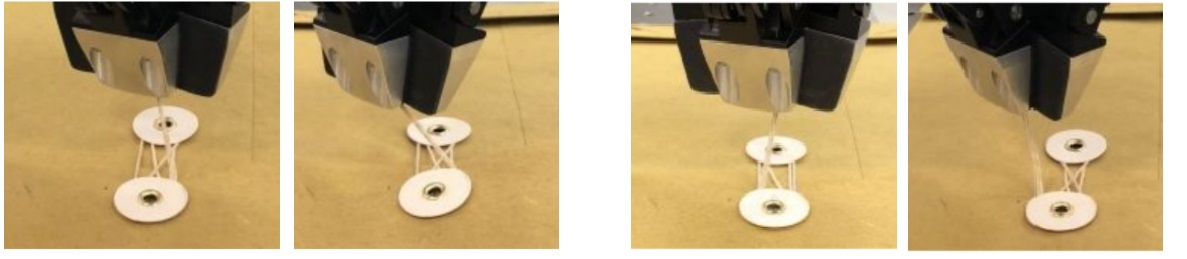
\includegraphics[height=35mm]{chapters/figures/experiments/exp2_CWCCW1.jpg}
	\caption{CW case on the left and CCW case on the right for r = 4 mm.}
	\label{fig:CWCCW1}
\end{figure}

Let's see the results for torques in Table~\ref{tab:4mm}.
% Table generated by Excel2LaTeX from sheet 'CW P1'
\begin{table}[htbp]
	\centering
	\begin{tabular}{|l|c|c|c|}
		\cmidrule{2-4}    \multicolumn{1}{r|}{} & \multicolumn{3}{c|}{\textbf{r = 4 mm}} \\
		\cmidrule{2-4}    \multicolumn{1}{r|}{} & \textbf{$|M_{x, tension} - M_{x, no tension}|$} & \textbf{$|M_{y, tension} - M_{y, no tension}|$} & Comparison to threshold \\
		\cmidrule{1-4}
		\textbf{CW case} & $0.101 N \cdot m$ & $0.142 N \cdot m$ & $> 0.095 N \cdot m$ \\
		\midrule
		\textbf{CCW case} & $0.053 N \cdot m$ & $0.018 N \cdot m$ & $< 0.095 N \cdot m$ \\
		\bottomrule
	\end{tabular}%
	\caption{Results for torque values in CW and CCW case for r = 4mm.}
	\label{tab:4mm}%
\end{table}%

We appreciate that when the gripper moves $2 \cdot r_{p}$ in perpendicular to pivots' joining axis in CW case both $|\Delta M_{x}|$ and $| \Delta M_{y}|$ are greater than threshold value while in CCW case they are smaller. We can thus distinguish both cases for a pivot's radius of 4 mm.

Let's see what happens with a radius of 3 mm.

\subsection{Radius = 3 mm}
For this experiment, we took a pen with a radius of 3 mm and we winded the string of the envelope around it CW and then CCW. Figure~\ref{fig:CWCCW2} shows both cases:
\begin{figure}[h!]
	\centering
	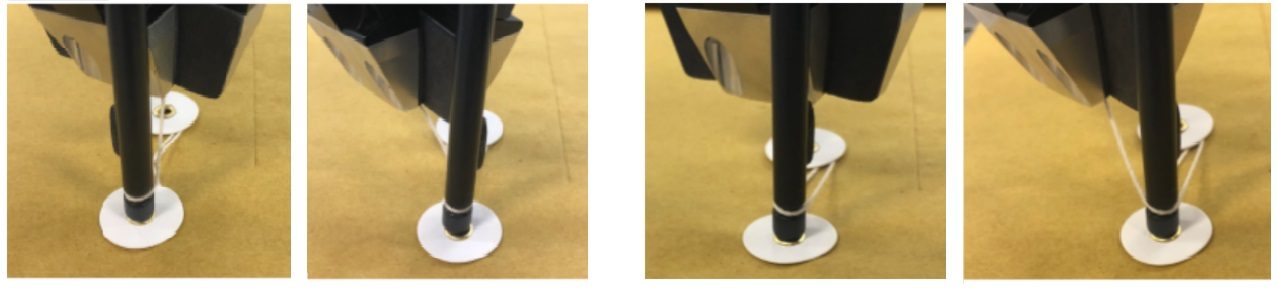
\includegraphics[height=35mm]{chapters/figures/experiments/exp2_CWCCW2.jpg}
	\caption{CW case on the left and CCW case on the right for r = 3 mm.}
	\label{fig:CWCCW2}
\end{figure}

Let's see the results for torques in Table~\ref{tab:3mm}.
% Table generated by Excel2LaTeX from sheet 'CW P1'
\begin{table}[htbp]
	\centering
	\begin{tabular}{|l|c|c|c|}
		\cmidrule{2-4}    \multicolumn{1}{r|}{} & \multicolumn{3}{c|}{\textbf{r = 3 mm}} \\
		\cmidrule{2-4}    \multicolumn{1}{r|}{} & \textbf{$|M_{x, tension} - M_{x, no tension}|$} & \textbf{$|M_{y, tension} - M_{y, no tension}|$} & Comparison to threshold \\
		\cmidrule{1-4}
		\textbf{CW case} & $0.254 N \cdot m$ & $0.185 N \cdot m$ & $> 0.095 N \cdot m$ \\
		\midrule
		\textbf{CCW case} & $0.020 N \cdot m$ & $0.056 N \cdot m$ & $< 0.095 N \cdot m$ \\
		\bottomrule
	\end{tabular}%
	\caption{Results for torque values in CW and CCW case for r = 3mm.}
	\label{tab:3mm}%
\end{table}%

We appreciate the same as in the previous case. In CW case both $|\Delta M_{x}|$ and $| \Delta M_{y}|$ are greater than threshold value while in CCW case they are smaller. We can thus distinguish both cases for a pivot's radius of 3 mm.

Let's see now what happens with a radius of 2 mm.

\subsection{Radius = 2 mm}
For this experiment, we took an Allen key with a 2 mm radius and we winded the string around it CW and then CCW. Both cases are shown in Figure~\ref{fig:CWCCW3}:
\begin{figure}[h!]
	\centering
	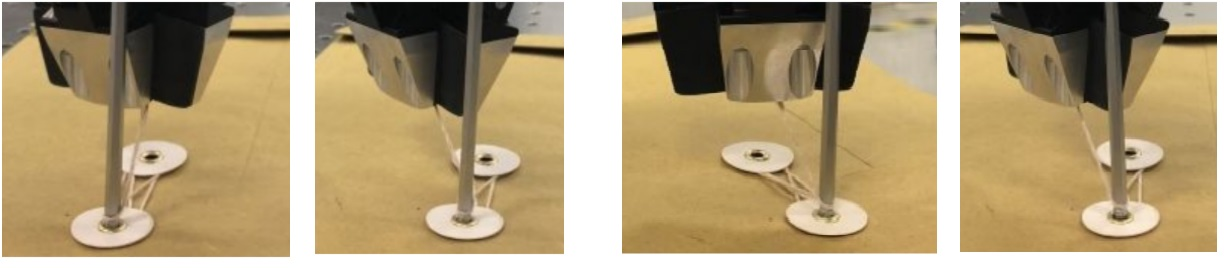
\includegraphics[height=35mm]{chapters/figures/experiments/exp2_CWCCW3.jpg}
	\caption{CW case on the left and CCW case on the right case for r = 2 mm.}
	\label{fig:CWCCW3}
\end{figure}

The results for torques are shown in Table~\ref{tab:2mm}.
% Table generated by Excel2LaTeX from sheet 'CW P1'
\begin{table}[htbp]
	\centering
	\begin{tabular}{|l|c|c|c|}
		\cmidrule{2-4}    \multicolumn{1}{r|}{} & \multicolumn{3}{c|}{\textbf{r = 2 mm}} \\
		\cmidrule{2-4}    \multicolumn{1}{r|}{} & \textbf{$|M_{x, tension} - M_{x, no tension}|$} & \textbf{$|M_{y, tension} - M_{y, no tension}|$} & Comparison to threshold \\
		\cmidrule{1-4}
		\textbf{CW case} & $0.405 N \cdot m$ & $0.320 N \cdot m$ & $> 0.095 N \cdot m$ \\
		\midrule
		\textbf{CCW case} & $0.566 N \cdot m$ & $0.407 N \cdot m$ & $> 0.095 N \cdot m$ \\
		\bottomrule
	\end{tabular}%
	\caption{Results for torque values in CW and CCW case for r = 2mm.}
	\label{tab:2mm}%
\end{table}%

In this case, we see that both in CW and CCW case, if the gripper moves $2 \cdot r_{p}$ in perpendicular to pivots' joining axis,  $|\Delta M_{x}|$ and $| \Delta M_{y}|$ are greater than threshold value. In this case we can thus not distinguish between CW and CCW case. For this algorithm to work with this force/torque sensor, pivots' radius must be bigger than 2 mm. A radius of 2 mm or smaller could be considered as negligible.

\section{Experiment 3: Minimum distance between pivots}
In this section we show different experiments where we modify the distance between pivots to figure out which is the minimum distance we could have for the force/torque sensor to distinguish between P1 and P2.

Let's start by analyzing what happens with the real distance between pivots (4.25 cm).

\subsection{Distance = 4.25 cm}
For this experiment, we first tied the string around P1 and then about P2 and we took torque values when the gripper moved $2 \cdot r_{p}$ in perpendicular to pivots' joining axis.

In Figure~\ref{fig:distance1} this first experiment is shown:
\begin{figure}[h!]
	\centering
	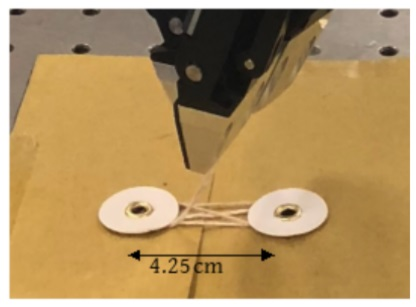
\includegraphics[height=40mm]{chapters/figures/experiments/exp3_distance1.jpg}
	\caption{First experiment with a distance of 4.25 cm between pivots.}
	\label{fig:distance1}
\end{figure}

Values for torques when the string is tied about P1 and when the string is tied about P2 are shown in Table~\ref{tab:distance1} below.
% Table generated by Excel2LaTeX from sheet 'CW P1'
\begin{table}[htbp]
	\centering
	\begin{tabular}{|l|c|c|c|c|}
		\cmidrule{2-5}    \multicolumn{1}{r|}{} & \multicolumn{4}{c|}{\textbf{d = 4.25 cm}} \\
		\cmidrule{2-5}    \multicolumn{1}{r|}{} & \multicolumn{1}{l|}{\textbf{$M_{x, no tension}$}} & \textbf{$M_{x, tension}$} & \textbf{$M_{x, tension} - M_{x, no tension}$} & Comparison to threshold \\
		\midrule
		\textbf{P1} & $0.026 N \cdot m$ & $-0.134 N \cdot m$ & $-0.160 N \cdot m$ & $< -0.095 N \cdot m$ \\
		\midrule
		\textbf{P2} & $-0.035 N \cdot m$ & $0.067 N \cdot m$ & $0.102 N \cdot m$ & $> 0.095 N \cdot m$ \\
		\bottomrule
	\end{tabular}%
	\caption{Results for torque values when the string is tied about P1 and about P2 for a distance of 4.25 cm between pivots.}
	\label{tab:distance1}%
\end{table}%

In the case where the string is tied about P1, $\Delta M_{x}$ is less than the negative value of the threshold when the gripper moves $2 \cdot r_{p}$, while when the string is tied about P2, $\Delta M_{x}$ is greater than the positive value of the threshold. We can thus distinguish if the string is tied about P1 or P2 for a distance of 4.25 cm between pivots (real case).

Let's see what happens for a distance of 3.5 cm between pivots.

\subsection{Distance = 3.5 cm}
For this experiment, we did the same thing as in the previous one but we changed pivots' distance to 3.5 cm. This is shown in Figure~\ref{fig:distance2} below:
\begin{figure}[h!]
	\centering
	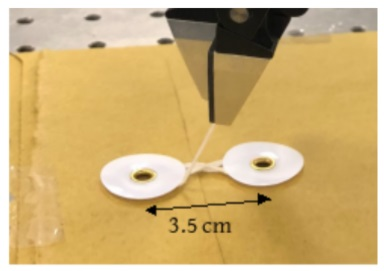
\includegraphics[height=40mm]{chapters/figures/experiments/exp3_distance2.jpg}
	\caption{Experiment with a distance of 3.5 cm between pivots.}
	\label{fig:distance2}
\end{figure}

Values for torques when the string is tied about P1 and when the string is tied about P2 are shown in Table~\ref{tab:distance2} below.
% Table generated by Excel2LaTeX from sheet 'CW P1'
\begin{table}[htbp]
	\centering
	\begin{tabular}{|l|c|c|c|c|}
		\cmidrule{2-5}    \multicolumn{1}{r|}{} & \multicolumn{4}{c|}{\textbf{d = 3.5 cm}} \\
		\cmidrule{2-5}    \multicolumn{1}{r|}{} & \multicolumn{1}{l|}{\textbf{$M_{x, no tension}$}} & \textbf{$M_{x, tension}$} & \textbf{$M_{x, tension} - M_{x, no tension}$} & Comparison to threshold \\
		\midrule
		\textbf{P1} & $0.004 N \cdot m$ & $-0.097 N \cdot m$ & $-0.101 N \cdot m$ & $< -0.095 N \cdot m$ \\
		\midrule
		\textbf{P2} & $-0.032 N \cdot m$ & $0.073 N \cdot m$ & $0.105 N \cdot m$ & $> 0.095 N \cdot m$ \\
		\bottomrule
	\end{tabular}%
	\caption{Results for torque values when the string is tied about P1 and about P2 for a distance of 3.5 cm between pivots.}
	\label{tab:distance2}%
\end{table}%

Again, in this case as in the previous one, when the string is tied about P1, $\Delta M_{x}$ is less than the negative value of the threshold, while when the string is tied about P2, $\Delta M_{x}$ is greater than the positive value of the threshold. We can thus distinguish whether the string is tied about P1 or P2 for a distance of 3.5 cm between pivots.

Let's see now what happens for a distance of 3 cm between pivots.

\subsection{Distance = 3 cm}
For this experiment, we changed pivots' distance to 3 cm. This is shown in Figure~\ref{fig:distance3} below:
\begin{figure}[h!]
	\centering
	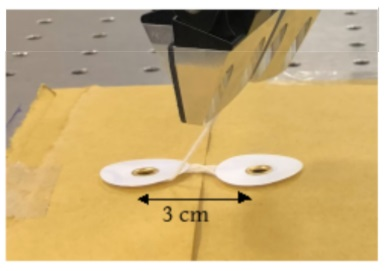
\includegraphics[height=40mm]{chapters/figures/experiments/exp3_distance3.jpg}
	\caption{Experiment with a distance of 3 cm between pivots.}
	\label{fig:distance3}
\end{figure}

Values for torques when the string is tied about P1 and when the string is tied about P2 are shown in Table~\ref{tab:distance3} below.
% Table generated by Excel2LaTeX from sheet 'CW P1'
\begin{table}[htbp]
	\centering
	\begin{tabular}{|l|c|c|c|c|}
		\cmidrule{2-5}    \multicolumn{1}{r|}{} & \multicolumn{4}{c|}{\textbf{d = 3 cm}} \\
		\cmidrule{2-5}    \multicolumn{1}{r|}{} & \multicolumn{1}{l|}{\textbf{$M_{x, no tension}$}} & \textbf{$M_{x, tension}$} & \textbf{$M_{x, tension} - M_{x, no tension}$} & Comparison to threshold \\
		\midrule
		\textbf{P1} & $0.033 N \cdot m$ & $-0.026 N \cdot m$ & $-0.007 N \cdot m$ & $> -0.095 N \cdot m$ \\
		\midrule
		\textbf{P2} & $0.032 N \cdot m$ & $0.046 N \cdot m$ & $0.014 N \cdot m$ & $< 0.095 N \cdot m$ \\
		\bottomrule
	\end{tabular}%
	\caption{Results for torque values when the string is tied about P1 and about P2 for a distance of 3 cm between pivots.}
	\label{tab:distance3}%
\end{table}%

In this case, when the string is tied about P1 as well as when it is tied about P2, $|\Delta M_{x}|$ is less than the the threshold value, when the gripper moves $2 \cdot r_{p}$. We can thus not know which pivot the string is tied about for a distance of 3 cm between pivots or less.

\section{Experiment 4: Comparison of robot fail ratio with human fail ratio}
For this experiment we performed 30 tests where the robot had to open the envelope that had been previously tied arbitrarily. Then, we performed this same 30 tests with 5 different human being with closed eyes, so they were in the same conditions than the robot. Finally we compared the results to see who succeed more times.

Let's start by seeing robot results of success and fails in Table~\ref{tab:exp4_robot}.
% Table generated by Excel2LaTeX from sheet 'CW P1'
\begin{table}[htbp]
	\centering
	\begin{tabular}{|l|c|}
		\cmidrule{2-2}    \multicolumn{1}{r|}{} & \textbf{Robot} \\
		\midrule
		\textbf{Success} & 19 \\
		\midrule
		\textbf{Fails} & 11 \\
		\bottomrule
	\end{tabular}%
	\caption{Number of success and fails made by the robot in the 30 experiments.}
	\label{tab:exp4_robot}%
\end{table}%

The robot succeded 19 times to open the envelope and failed 11 out of 30 attempts. The reasons why the robot failed are:
\begin{itemize}
 \item Bad reading of the torque by the sensor: a bad reading of torque makes the robot to take the wrong action. For example, it turns around the wrong pivot or in the wrong direction.
 \item Error in the movement of the robot: if there is an error in the movement and the spiral movement is not perfect, the gripper may pull the string too much during the movement (and break it) or it may not finish the turn where it is supposed to and the envelope will not be opened.
\end{itemize}

Let's see now the results for humans. In Figure~\ref{fig:humans} we can see how the experiment was performed by the 5 people:
\begin{figure}[h!]
	\centering
	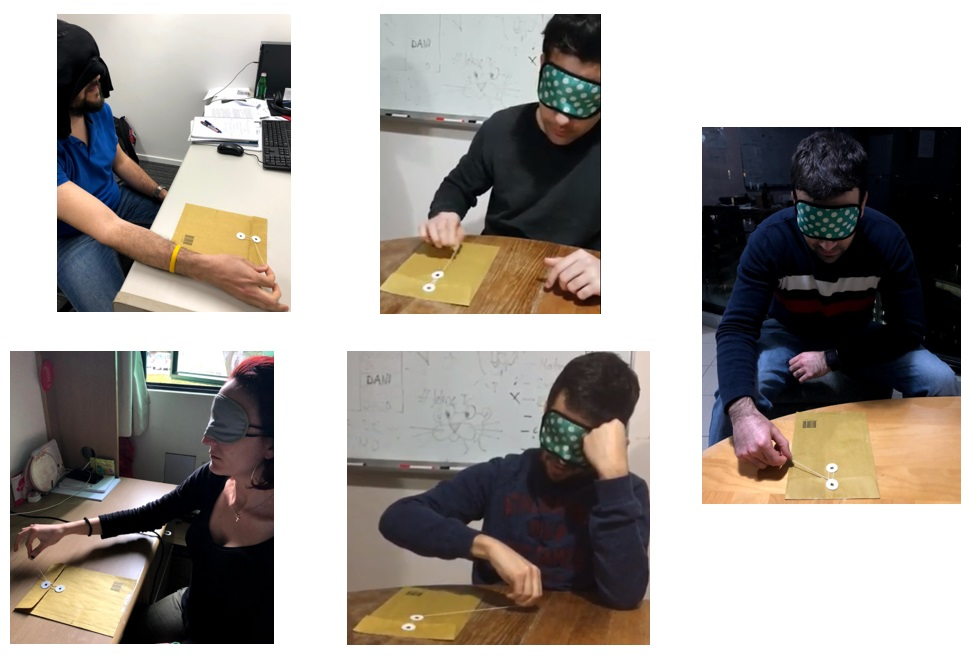
\includegraphics[height=80mm]{chapters/figures/experiments/exp4_humans.jpg}
	\caption{Experiment performed by 5 people with closed eyes trying to open the envelope.}
	\label{fig:humans}
\end{figure}

In Table~\ref{tab:humans}, the results for these 5 people are shown:\newline
% Table generated by Excel2LaTeX from sheet 'CW P1'
\begin{table}[h!]
	\centering
	\begin{tabular}{|l|c|c|c|c|c|}
		\cmidrule{2-6}    \multicolumn{1}{r|}{} & \textbf{Human 1} & \textbf{Human 2} & \textbf{Human 3} & \textbf{Human 4} & \textbf{Human 5} \\
		\midrule
		\textbf{Success} & 12    & 21    & 17    & 7     & 26 \\
		\midrule
		\textbf{Fails} & 18    & 9     & 13    & 23    & 4 \\
		\bottomrule
	\end{tabular}%
	\caption{Number of success and fails made by the 5 people in the 30 experiments.}
	\label{tab:humans}%
\end{table}%

We appreciate that results for different humans are very different. That is why we took different people to perform the experiments, because every person is different while the algorithm for the robot will always work the same way.
The reasons why people failed are:
\begin{itemize}
	\item They did not know which direction to turn.
	\item They did not know where they were in the space and they gave up.
	\item They thought the envelope was already opened and it was not.
\end{itemize}

Let's compare now the percentage of success for the robot and for an average person in Table~\ref{tab:comprobothuman}:
% Table generated by Excel2LaTeX from sheet 'CW P1'
\begin{table}[htbp]
	\centering
	\begin{tabular}{|l|c|c|}
		\cmidrule{2-3}    \multicolumn{1}{r|}{} & \textbf{Robot} & \textbf{Humans} \\
		\midrule
		\textbf{Percentage of success} & 63.30\% & 55.30\% \\
		\bottomrule
	\end{tabular}%
	\caption{Comparison between robot percentage of success and human percentage of success.}
	\label{tab:comprobothuman}%
\end{table}%

We see that the percentage of success for the robot is higher than for an average human. 

The main difference between humans and the robot was that people could correct their movement if they realized they were doing it wrong, while the robot is not able to correct the movement and will not open the envelope if it doesn't figure out the good movement the first time.

We also noticed that when a person succeded to open the envelope, he or she took much less time than the robot. The robot takes around 4 minutes to open the envelope while the human did it in about 30 seconds.
